\begin{chapter}{\label{cha:bose_gases}Introduction}
In quantum mechanics there are two classes of particle: bosons and fermions. Fermionic particles (such as electrons) follow Fermi-Dirac statistics, have half-integer spin, and obey the Pauli exclusion principle. Bosonic particles (such as photons) have integer spin, follow Bose-Einstein statistics and, unlike fermions, any number are permitted to occupy the same quantum state. Under certain conditions, this latter property allows a large fraction of bosons to occupy the ground state macroscopically, a phenomenon known as Bose-Einstein condensation (BEC) \cite{Pethick,stringari}. Bose-Einstein condensation is as diverse as it is astonishing, appearing in all manner of topics from atomic physics to condensed matter to astrophysics, manifesting as unexpected phenomena such as superfluidity, quantised circulation and superconductivity \cite{griffin1996bose,tilley1990superfluidity}. These effects derive directly from quantum mechanics, and the fluids that exhibit them are known as ``quantum fluids''.

\section{Bose-Einstein condensation}\label{section:becinintro}
The roots of the original prediction of Bose-Einstein condensation lies with Indian scientist, Satyendra Nath Bose. In 1924 Bose re-derived Planck's law of black-body radiation, developing a theory of the statistical mechanics of photons by treating them as a collection of identical particles \cite{bose}. Albert Einstein helped Bose publish his work and went on to generalise his photon distribution law to an ideal gas of $N$ non-interacting massive bosons \cite{Einstein24}. This led to the Bose-Einstein distribution, $f(\epsilon_i)$, describing the statistical distribution of bosons over single particle energy states,
\begin{equation}
	f(\epsilon_i) = \frac{1}{e^{(\epsilon_i - \mu) / k_{\rm B}T} - 1},
\end{equation}
where $\epsilon_i$ is the energy of level $i$, $\mu$ is the chemical potential, $k_{\rm B}$ is the Boltzmann constant, and T is the temperature. The total number of particles in the system can be written as a sum over the mean occupation of each energy level,
\begin{equation}
	N = \sum\limits_i N_i = \sum\limits_i g(\epsilon_i)f(\epsilon_i),
\end{equation}
where $N_i$ is the mean occupation of level $i$ and $g(\epsilon_i)$ is the degeneracy of energy level $i$. Under the Bose-Einstein distribution the occupation of the ground state diverges in the limit of zero temperature, leading to the macroscopic occupation that defines the BEC. Schematically, Bose-Einstein condensation is shown in Figure \ref{fig:beclevels}. While it is impossible to reach the limit of $T=0$ in reality, the macroscopic occupation occurs for temperatures less than a certain critical value $T<T_\lambda$.

\begin{figure}
\centering
    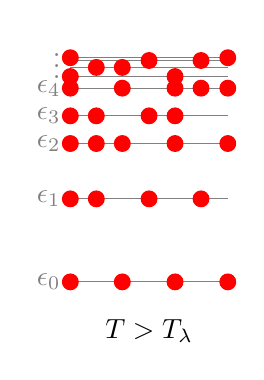
\begin{tikzpicture}
    \draw[gray] (2cm,0em) -- (0cm,0em) node[left] {$\epsilon_0$};
    \draw[gray] (2cm,3em) -- (0cm,3em) node[left] {$\epsilon_1$};
    \draw[gray] (2cm,5em) -- (0cm,5em) node[left] {$\epsilon_2$};
    \draw[gray] (2cm,6em) -- (0cm,6em) node[left] {$\epsilon_3$};
	\draw[gray] (2cm,7em) -- (0cm,7em) node[left] {$\epsilon_4$};
	\draw[gray] (2cm,7.42em) -- (0cm,7.42em) node[left] {$ $};
	\draw[gray] (2cm,7.75em) -- (0cm,7.75em) node[left] {$ $};
	\draw[gray] (2cm,8em) -- (0cm,8em) node[left] {$ $};
	\draw[gray] (2cm,8.1em) -- (0cm,8.1em) node[left] {$\vdots$};
	\draw[red,fill=red] (0.66cm,0em) circle (0.1cm);
	\draw[red,fill=red] (1.33cm,0em) circle (0.1cm);
	\draw[red,fill=red] (0cm,0em) circle (0.1cm);
	\draw[red,fill=red] (2cm,0em) circle (0.1cm);
	\draw[red,fill=red] (0cm,3em) circle (0.1cm);
	\draw[red,fill=red] (0.33cm,3em) circle (0.1cm);
	\draw[red,fill=red] (1cm,3em) circle (0.1cm);
	\draw[red,fill=red] (1.66cm,3em) circle (0.1cm);
	\draw[red,fill=red] (0cm,5em) circle (0.1cm);
	\draw[red,fill=red] (0.33cm,5em) circle (0.1cm);
	\draw[red,fill=red] (0.66cm,5em) circle (0.1cm);
	\draw[red,fill=red] (1.33cm,5em) circle (0.1cm);
	\draw[red,fill=red] (2cm,5em) circle (0.1cm);
	\draw[red,fill=red] (0cm,6em) circle (0.1cm);
	\draw[red,fill=red] (0.33cm,6em) circle (0.1cm);
	\draw[red,fill=red] (1cm,6em) circle (0.1cm);
	\draw[red,fill=red] (1.33cm,6em) circle (0.1cm);
	\draw[red,fill=red] (0cm,7em) circle (0.1cm);
	\draw[red,fill=red] (0.66cm,7em) circle (0.1cm);
	\draw[red,fill=red] (1.33cm,7em) circle (0.1cm);
	\draw[red,fill=red] (1.66cm,7em) circle (0.1cm);
	\draw[red,fill=red] (2cm,7em) circle (0.1cm);
	\draw[red,fill=red] (0cm,7.42em) circle (0.1cm);
	\draw[red,fill=red] (0.33cm,7.75em) circle (0.1cm);
	\draw[red,fill=red] (0.66cm,7.75em) circle (0.1cm);
	\draw[red,fill=red] (1cm,8em) circle (0.1cm);
	\draw[red,fill=red] (1.33cm,7.42em) circle (0.1cm);
	\draw[red,fill=red] (1.66cm,8em) circle (0.1cm);
	\draw[red,fill=red] (2cm,8.1em) circle (0.1cm);
	\draw[red,fill=red] (0cm,8.1em) circle (0.1cm);
	\draw (1cm,-1em) node[below] {$T>T_\lambda$};
    \end{tikzpicture}
    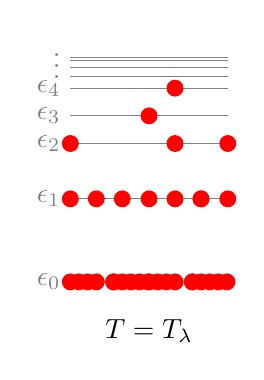
\begin{tikzpicture}
    \draw[gray] (2cm,0em) -- (0cm,0em) node[left] {$\epsilon_0$};
    \draw[gray] (2cm,3em) -- (0cm,3em) node[left] {$\epsilon_1$};
    \draw[gray] (2cm,5em) -- (0cm,5em) node[left] {$\epsilon_2$};
    \draw[gray] (2cm,6em) -- (0cm,6em) node[left] {$\epsilon_3$};
	\draw[gray] (2cm,7em) -- (0cm,7em) node[left] {$\epsilon_4$};
	\draw[gray] (2cm,7.42em) -- (0cm,7.42em) node[left] {$ $};
	\draw[gray] (2cm,7.75em) -- (0cm,7.75em) node[left] {$ $};
	\draw[gray] (2cm,8em) -- (0cm,8em) node[left] {$ $};
	\draw[gray] (2cm,8.1em) -- (0cm,8.1em) node[left] {$\vdots$};
	\draw[red,fill=red] (0cm,0em) circle (0.1cm);
	\draw[red,fill=red] (0.33cm,0em) circle (0.1cm);
	\draw[red,fill=red] (0.11cm,0em) circle (0.1cm);
	\draw[red,fill=red] (0.22cm,0em) circle (0.1cm);
	\draw[red,fill=red] (0.55cm,0em) circle (0.1cm);
	\draw[red,fill=red] (0.55cm,0em) circle (0.1cm);
	\draw[red,fill=red] (0.66cm,0em) circle (0.1cm);
	\draw[red,fill=red] (0.77cm,0em) circle (0.1cm);
	\draw[red,fill=red] (0.88cm,0em) circle (0.1cm);
	\draw[red,fill=red] (0.99cm,0em) circle (0.1cm);
	\draw[red,fill=red] (1cm,0em) circle (0.1cm);
	\draw[red,fill=red] (1.33cm,0em) circle (0.1cm);
	\draw[red,fill=red] (1.11cm,0em) circle (0.1cm);
	\draw[red,fill=red] (1.22cm,0em) circle (0.1cm);
	\draw[red,fill=red] (1.55cm,0em) circle (0.1cm);
	\draw[red,fill=red] (1.55cm,0em) circle (0.1cm);
	\draw[red,fill=red] (1.66cm,0em) circle (0.1cm);
	\draw[red,fill=red] (1.77cm,0em) circle (0.1cm);
	\draw[red,fill=red] (1.88cm,0em) circle (0.1cm);
	\draw[red,fill=red] (1.99cm,0em) circle (0.1cm);
	\draw[red,fill=red] (0cm,3em) circle (0.1cm);
	\draw[red,fill=red] (0.33cm,3em) circle (0.1cm);
	\draw[red,fill=red] (0.66cm,3em) circle (0.1cm);
	\draw[red,fill=red] (1cm,3em) circle (0.1cm);
	\draw[red,fill=red] (1.33cm,3em) circle (0.1cm);
	\draw[red,fill=red] (1.66cm,3em) circle (0.1cm);
	\draw[red,fill=red] (1.66cm,3em) circle (0.1cm);
	\draw[red,fill=red] (2cm,3em) circle (0.1cm);
	\draw[red,fill=red] (0cm,5em) circle (0.1cm);
	\draw[red,fill=red] (1.33cm,5em) circle (0.1cm);
	\draw[red,fill=red] (2cm,5em) circle (0.1cm);
	\draw[red,fill=red] (1cm,6em) circle (0.1cm);
	\draw[red,fill=red] (1.33cm,7em) circle (0.1cm);
	\draw (1cm,-1em) node[below] {$T=T_\lambda$};
  \end{tikzpicture}
  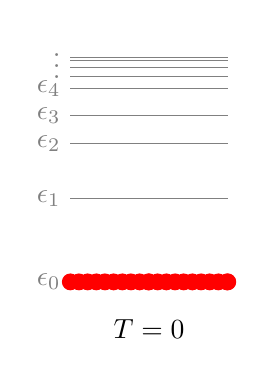
\begin{tikzpicture}
    \draw[gray] (2cm,0em) -- (0cm,0em) node[left] {$\epsilon_0$};
    \draw[gray] (2cm,3em) -- (0cm,3em) node[left] {$\epsilon_1$};
    \draw[gray] (2cm,5em) -- (0cm,5em) node[left] {$\epsilon_2$};
    \draw[gray] (2cm,6em) -- (0cm,6em) node[left] {$\epsilon_3$};
	\draw[gray] (2cm,7em) -- (0cm,7em) node[left] {$\epsilon_4$};
	\draw[gray] (2cm,7.42em) -- (0cm,7.42em) node[left] {$ $};
	\draw[gray] (2cm,7.75em) -- (0cm,7.75em) node[left] {$ $};
	\draw[gray] (2cm,8em) -- (0cm,8em) node[left] {$ $};
	\draw[gray] (2cm,8.1em) -- (0cm,8.1em) node[left] {$\vdots$};
	\draw[red,fill=red] (0cm,0em) circle (0.1cm);
	\draw[red,fill=red] (0.33cm,0em) circle (0.1cm);
	\draw[red,fill=red] (0.11cm,0em) circle (0.1cm);
	\draw[red,fill=red] (0.22cm,0em) circle (0.1cm);
	\draw[red,fill=red] (0.44cm,0em) circle (0.1cm);
	\draw[red,fill=red] (0.55cm,0em) circle (0.1cm);
	\draw[red,fill=red] (0.66cm,0em) circle (0.1cm);
	\draw[red,fill=red] (0.77cm,0em) circle (0.1cm);
	\draw[red,fill=red] (0.88cm,0em) circle (0.1cm);
	\draw[red,fill=red] (0.99cm,0em) circle (0.1cm);
	\draw[red,fill=red] (1cm,0em) circle (0.1cm);
	\draw[red,fill=red] (1.33cm,0em) circle (0.1cm);
	\draw[red,fill=red] (1.11cm,0em) circle (0.1cm);
	\draw[red,fill=red] (1.22cm,0em) circle (0.1cm);
	\draw[red,fill=red] (1.55cm,0em) circle (0.1cm);
	\draw[red,fill=red] (1.44cm,0em) circle (0.1cm);
	\draw[red,fill=red] (1.66cm,0em) circle (0.1cm);
	\draw[red,fill=red] (1.77cm,0em) circle (0.1cm);
	\draw[red,fill=red] (1.88cm,0em) circle (0.1cm);
	\draw[red,fill=red] (1.99cm,0em) circle (0.1cm);
	\draw[red,fill=red] (2cm,0em) circle (0.1cm);
	\draw (1cm,-1em) node[below] {$\phantom{T_\lambda}T=0\phantom{T_\lambda}$};
  \end{tikzpicture}
  \caption{\label{fig:beclevels}Schematic depiction of Bose-Einstein condensation. The ground state $\epsilon_0$ becomes macroscopically occupied as the temperature is reduced to below the critical temperature for condensation. In the limit of $T=0$ all bosons occupy the ground state.}
\end{figure}

Consider a gas of non-interacting bosons in thermal equilibrium at temperature $T$. The thermal de Broglie wavelength for each particle characterises the spatial extent of its localised wavepacket, and is conventionally defined by
\begin{equation}
\lambda_{\rm dB} = \sqrt{\frac{2\pi \hbar^2}{mk_{\rm B}T}},
\label{eq:debroglie}
\end{equation}
where $m$ is the mass of the particle and $\hbar$ is the reduced Plank constant. The de Broglie wavelength is inversely proportional to the square root of the temperature $T$, so that at high temperatures the wavepacket of each particle is small compared to the average inter-particle distance. Here classical, particle-like behaviour dominates the dynamics of the gas and the particles approximately follow the classical Boltzmann distribution. As the temperature of the gas is reduced, the wavelength associated with the particles grows. At a critical temperature, $T_\lambda$, the wavelength for each particle becomes comparable to the average inter-particle distance and the individual characteristics of particles are no longer apparent. Here the particles become indistinguishable and the idea of a particle trajectory no longer makes sense. The particles behave in a truly quantum manner and form a degenerate gas. The critical temperature for which this process occurs marks the onset of Bose-Einstein condensation.

For a gas of identical non-interacting Bosons in a uniform three-dimensional system of volume $V$ and number density $n=N/V$, Bose-Einstein condensation occurs when $n\lambda_{\rm dB}^3 \leq \zeta(3/2)$ \cite{Pethick,huang1987statistical}, where $\zeta(3/2)\approx2.612$ is the Riemann zeta function evaluated at $3/2$. By using this relation with Equation \ref{eq:debroglie} one finds the critical temperature,
\begin{equation}
T_\lambda = \frac{2\pi\hbar^2}{mk_{\rm B}} \left ( \frac{n}{\zeta(3/2)} \right )^{2/3},
\label{eq:tlambda}
\end{equation}
for the onset of Bose-Einstein condensation. The fraction of bosons condensed into the ground state, termed the condensate fraction, then be calculated as a function of temperature,
\begin{equation}
	\frac{N_0}{N} = 1 - \left( \frac{T}{T_\lambda}\right )^{3/2}.
\end{equation}

\section{Superfluid helium}
Many concepts relating to Bose-Einstein condensation and quantum gases were developed in the context of liquid $^4$He. Liquid helium is interesting in that when cooled to very low temperatures, the liquid does not crystallise or solidify at atmospheric pressures. In fact a pressure of over $25$ atmospheres is required to solidify $^4$He, even at its lowest temperatures \cite{Pethick}. 

Around 1930, Keesom {\it et. al} \cite{Keesom27,Keesom35} observed that when cooling liquid $^4$He, there exists a critical temperature known as the lambda point ($T_\lambda = 2.17$ K) at which the fluid undergoes a phase transition into a state known as helium II. It was later discovered by Kapitza \cite{Kapitza}, Allen and Misener \cite{Allen38} that helium II exhibits inviscid flow (one of several remarkable properties of helium II), and the fluid was deemed a ''superfluid''.

London \cite{London38,London38b} was the first to interpret the properties of helium II as a manifestation of Bose-Einstein condensation of helium atoms, but the idea was not widely accepted at first. The strongly-interacting liquid of helium atoms is a world away from Einstein's non-interacting gas of bosons. Instead, the two-fluid model of Landau \cite{Landau41} was the first successful description of helium II hydrodynamics, wherein two fluids exist alongside one another with densities depending on the temperature: an inviscid superfluid component and a viscous normal fluid component. At $T=T_\lambda$, the normal fluid makes up the entire fluid and there is no superfluid component. As the temperature is decreased, the proportion of the normal fluid decreases and that of the superfluid increases, such that at $T=0$ the fluid is entirely superfluid.

\subsection{Dispersion relation and excitations}
Landau showed that superfluid behaviour can be accounted for by a dispersion relation that is linear at low momenta \cite{Landau41}. Bogoliubov then showed that a weakly-interacting Bose gas supports exactly such a dispersion law \cite{bogo47}. This link between bosonic gases and helium II was a strong indicator that Bose-Einstein condensation was indeed the fundamental mechanism behind superfluidity, and finally gave traction to London's theory. Onsager \cite{Onsager49} and Feynman \cite{Feynman55} then predicted quantised circulation as an extension to London's work.

While Bose-Einstein condensation is now known to be the driving force behind helium II superfluidity, the strong interactions inherent in liquid helium restricts the condensed fraction of helium atoms to less than $10\%$ \cite{Donnelly} (even in the limit of zero temperature) and so a weakly-interacting Bose gas provides only a qualitative model of helium II superfluidity.

\begin{figure}
	\centering
	\begin{tikzpicture}
		\begin{axis}[samples=300,ylabel near ticks,xlabel near ticks,
				width=0.4\linewidth,
				height=0.45\linewidth,
				xlabel=$p$,
				ylabel=$\epsilon$,
				xmin=0,
				xmax=13,
				ymin=0.4,
				ymax=12,
				axis line style={-Latex[round]},
				axis y line*=left,
        axis x line*=bottom,
        yticklabels={,,},
        xticklabels={,,},
				major tick length = 0.00cm]
				\addplot[mark=none,thick,domain=0:12] {x^(0.25)*((x/2-4)*sin(deg(x/2-4)) + 4)};
		\end{axis}
	\end{tikzpicture}%
	\caption{\label{fig:hedisp}The dispersion relation for superfluid $^4$He, demonstrating the spectrum of elementary excitations. The linear dispersion of phonons can be seen at low momenta and the roton minimum at higher momenta.}
\end{figure}

The dispersion relation for liquid helium $^4$He is shown in Figure \ref{fig:hedisp}. For small momenta the relation is indeed linear. The fundamental excitations associated with this part of the relation are sound waves, known as {\it phonons}. For larger momentum, however, $\epsilon(p)$ exhibits an approximately quadratic shaped dip and local minimum. The fundamental excitations of this part of the relation are known as {\it rotons}, with the centre of the dip corresponding to the smallest possible energy of a roton, the {\it roton minimum}. 

\section{Dilute weakly-interacting atomic gases}
Gases of alkali atoms such as rubidium, sodium and lithium are ideal candidates for condensation: they are weakly-interacting, can be easily trapped magnetically, and readily cooled using lasers. When considering these gases, Einstein's ideal gas predictions provide a good estimate of the critical temperature for Bose-Einstein condensation.  However, as the gas is cooled towards the critical temperature it is necessary to avoid the transition into a liquid or solid. This can be done by reducing the atomic density such that the gas is dilute enough that elastic binary collisions in the gas dominate over three-body collisions. The required atomic densities are around $n \sim 10^{14}~{\rm cm}^{-3}$ \footnote{Compare this to the density of dry air at room temperature and pressure, $n \sim 10^{19}~{\rm cm}^{-3}$.}, and so by using Equation \ref{eq:tlambda} one predicts that the ultra-low temperatures of $T \sim 10^{-6}~{\rm K}$ are required for the onset of Bose-Einstein condensation.

\subsection{Experimental realisation}
The requirement of such low temperatures delayed the realisation of a true atomic BEC until 1995, when advances in atom cooling and trapping \cite{billphillips,chu98,Cohen-Tannoudji} lead to the condensation in vapours of rubidium ($^{87}$Rb) by the group of Professors Carl Wieman and Eric Cornell at the University of Colorado \cite{Anderson198}, and sodium ($^{23}$Na) by the group of W. Ketterle at MIT \cite{PhysRevLett.75.3969}. Wieman, Cornell and Ketterle were awarded the 2001 Nobel Prize in Physics for ``{\it the achievement of Bose-Einstein condensation in dilute gases of alkali atoms, and for early fundamental studies of the properties of the condensates}'' \cite{nobel01}.

A variety of cooling techniques, including laser \cite{billphillips,chu98,Cohen-Tannoudji} and evaporative \cite{PhysRevB.34.3476} cooling, originally developed in the attempt to condense spin-polarised hydrogen \cite{Hecht59, PhysRevLett.44.164, Silvera86}, are used to reach the ultra-low temperatures required for atomic Bose-Einstein condensation \cite{Pethick,RevModPhys.74.1131,RevModPhys.74.875}. A typical atomic condensate begins life as around $10^9$ atoms which are cooled to around 1K by a Zeeman slower: a laser beam propagating opposite to the atom flow reduces the velocity of the atoms from around $800~\rm{m/s}$ to $30~\rm{m/s}$. The atoms are transferred to a magneto-optical trap (MOT) formed by laser beams and magnetic fields and further cooled through Doppler cooling, where the Doppler effect is employed to reduce the momentum of atoms. A limit of this method is reached at around $1\,\mu$K \cite{Pethick} at which point evaporative cooling is required to cool the gas even further. Here the confining trap is carefully modified so that the high energy atoms escape the system. The remaining lower energy atoms rethermalise at a reduced temperature and lower density due to the loss of atoms. Using this technique, the gas can be cooled to the nK regime. The BEC then emerges marked by a very narrow velocity distribution for the atoms, indicating a macroscopic occupation of the ground state. 

Since the first experiments in 1995, an explosion of ultra-cold atomic physics has followed. Many species of atom are now routinely condensed by over 100 experimental groups all over the world. The list grows continuously: many alkalis \cite{Anderson198,PhysRevLett.75.3969,PhysRevLett.75.1687,PhysRevLett.78.985,PhysRevLett.85.1795,Modugno,Robert461,Weber232}, calcium \cite{PhysRevLett.103.130401}, dysprosium \cite{PhysRevLett.107.190401}, strontium \cite{PhysRevLett.103.200401,PhysRevLett.103.200402, PhysRevA.82.041602, PhysRevA.81.051601}, ytterbium \cite{PhysRevLett.91.040404}, chromium \cite{PhysRevLett.94.160401}, spin-polarised hydrogen \cite{PhysRevLett.81.3811}, metastable helium \cite{PhysRevLett.86.3459}, magnons \cite{Mathew11}, exciton-polaritons \cite{Kasprzak06} and even mixtures of different species \cite{PhysRevLett.89.053202, PhysRevLett.89.190404, PhysRevLett.100.210402,PhysRevA.84.011603}. Each species expands the richness of the fascinating phenomena available to experimentalists, with their unique atomic properties and range of interactions.

The experimental advances of controlling the trapping potential has allowed for direct interaction with the condensate using time-dependent magnetic fields and lasers. Localised laser beams can punch a `hole' in a condensate to create almost arbitrarily shaped obstacles \cite{Henderson09}. Exotic trapping potentials such as ring traps \cite{persistent,Ramanathan11}, uniform box traps \cite{gaunt_2013,chomaz_2015}, optical lattices \cite{Greiner02} and double-well \cite{PhysRevLett.106.025302} potentials can be realised with relative ease. The route has even opened to experimentation in reduced dimensionality \cite{Gorlitz,PhysRevLett.87.080403,PhysRevLett.91.250402,PhysRevLett.92.173003}. By significantly trapping the gas along one dimension it is possible to make a disc shaped, effectively two dimensional condensate, useful \cite{Neely,Freilich2010} for the study of vortex dynamics. A further trapping along a second dimension creates an elongated, effectively one dimensional condensate such that solitons, one-dimensional non-dispersive waves, become supported \cite{drazin1989solitons,PhysRevLett.101.120406}.

\subsection{Scattering length and interactions}
The atomic binary collisions in ultra-cold dilute gases are characterised by the $s$-wave scattering length, $a_s$. Higher energy $p$-wave and $d$-wave scattering is suppressed. Geometrically, a positive $a_s$ (as in a rubidium or sodium BEC) can be thought of as a measure of the effective radius of repulsive atoms. For gases with density in the region required, $n^{1/3}a_s \ll 1$, and so $a_s$ is much smaller than the average inter-atomic distance. This implies that the gas is weakly-interacting and around $99\%$ of the atoms can become Bose-condensed, resulting in a condensate fraction much greater than the theoretical maximum for helium II. This makes ultra-cold dilute atomic gases the purest form of BEC that can also be easily controlled and manipulated in the lab.

The scattering length may also be negative (as in a lithium BEC \cite{PhysRevLett.75.1687, PhysRevLett.78.985}). In this case the atoms are attractive, rather than repulsive, and the BEC is only stable up to a certain atom number. Importantly, it is possible to control the inter-atomic interaction, and therefore the scattering length, through the entire range of the parameter space using techniques such as {\it Feshbach resonance} (theoretically laid out in \cite{weiner2003cold} and experimentally demonstrated in \cite{Inouye1998,PhysRevLett.82.2422,PhysRevLett.85.1795}), providing further experimental control over the BEC.

With the unique level of purity and control available in the lab, weakly-interacting dilute atomic gases have become the ideal test-bed for studying Bose-Einstein condensation and for observation of quantum effects on a macroscopic scale.


\section{Macroscopic nonlinear excitations: vortices and solitons}
The rise of interest in Bose-Einstein condensation has led to a great amount of theoretical work. It can be argued that the greatest success in this area is the development of an effective mean-field theory which provides the so-called Gross-Pitaevskii equation (GPE) \cite{Pethick,Pitaevskii61,Gross61,RevModPhys.71.463}, a classical evolution equation and a variant of the nonlinear-Schr\"odinger equation used in many areas of physics, including plasma physics \cite{PhysRevLett.37.693} and non-linear optics \cite{PhysRevA.65.053614,borisSolitons}. The GPE is much simpler than modelling a BEC using the full many-body Schr\"oedinger equation, yet accurately captures the statics and dynamics \cite{RevModPhys.71.463,Denschlag97, Burger99, PhysRevLett.86.2926, Dutton27072001,vortices,lobo_2004,PhysRevLett.85.2857} of a BEC over a range of realistic experimental parameters. Section \ref{cha:theoretical_model} describes the mean-field formulation  in detail and formally derives the GPE from the starting point of the many-body Schr\"oedinger equation.

The non-linearity in the GPE arises from atom-atom interactions and gives rise to a great deal of interesting effects, both from a mathematical standpoint and when modelling an atomic BEC. A selection of the interesting and experimentally relevant non-linear phenomena are described in this section.

\subsection{Vortices}
A family of non-linear excitations supported by the GPE are {\it quantum vortices}, which arise via topological defects in the wavefunction that parametrises the condensate. Solutions with quantum vortices contain structures identified by a localised density dip, the vortex core, masking a phase singularity in its centre. The phase singularity forms a velocity field such that fluid circulates around the vortex core.

Quantum vortices are carriers of vorticity in an irrotational superfluid system, and can arise both naturally during the formation of a BEC or by direct interaction with a condensate. A standard method of generating vortices, relevant to atomic condensates and helium II, is by rotation of the superfluid \cite{PhysRevLett.43.214,PhysRevLett.84.806,hodby_2002,Abo-Shaeer476, PhysRevLett.87.210403}. At lower angular speeds the rotation has no effect, however, above a critical value the presence of vortices lowers the energy of the system \cite{0953-8984-13-12-201,NozieresPines}. In this case, one or more vortices nucleate into the system, forming a lattice \cite{PhysRevLett.43.214,Abo-Shaeer476} at the centre of rotation. Another example is the formation of vortices as a result of broken symmetry after a fast quench into the BEC regime. Through the Kibble-Zurek mechanism \cite{0305-4470-9-8-029,Zurek85,KZvort99}, pockets of phase coherence form, separated in space. As the phase coherence grows in the condensate, boundaries are created and discontinuities along these boundaries leads to the formation of vortex lines. Further methods of generating vortices include artificial phase imprinting \cite{Cornell99,Dobrek99,Leanhardt99} of the topological defect via laser light, or by stirring a BEC with a localised laser beam \cite{PhysRevLett.84.806,hodby_2002,Abo-Shaeer476,jma00,Raman01,Inouye}.

Quantised vortices have much in common with the classical vortices observed in nature. However, while classical vortices can be created with any degree of fluid rotation, characterised by the circulation $\Gamma$, quantised vortices differ in that their circulation is constrained (as a direct consequence of quantum mechanics) to integer multiples of the {\it quantum of circulation}, $\kappa$, with a value dependent on the system.

Experimentally, quantum vortices have been observed in many different configurations and for various trap geometries. Quantised vortex lines \cite{Dutton27072001}, vortex rings \cite{PhysRevLett.86.2926}, vortex tangles \cite{Henn}, quasi-two-dimensional turbulence \cite{kwon_moon_14}, vortex lattices \cite{PhysRevLett.84.806,Abo-Shaeer476,abo_shaeer_2002,PhysRevLett.86.4443}, vortex dipoles \cite{Neely}, giant vortices \cite{PhysRevLett.90.170405}, and multiply charged vortices \cite{PhysRevLett.93.160406} have all been realised in BECs. The condensate is observed via imaging of the atomic gas density, but the vortex core size is typically smaller than the imaging resolution. To overcome this the condensate is expanded by releasing it from the trap prior to imaging. The vortices then appear as localized regions of low density in the expanded condensate images.

Quantum vortices have also been observed in superfluid helium \cite{Vinen218}. In 1979, the first clear and direct image of a quantised vortex lattice in rotating helium II was provided by Packard {\it et. al} \cite{PhysRevLett.43.214}. Electrons were trapped inside vortex cores and accelerated towards a florescent screen to mark the position of the vortex. The resulting images are shown in Figure \ref{fig:hevorts} for different rotation speeds. More recently, there has been a significant advance by Lathrop {\it et al} \cite{Bewley09}. Here vortex lines were visualised and tracked in helium II by using tracer particles of frozen hydrogen.

\begin{figure}
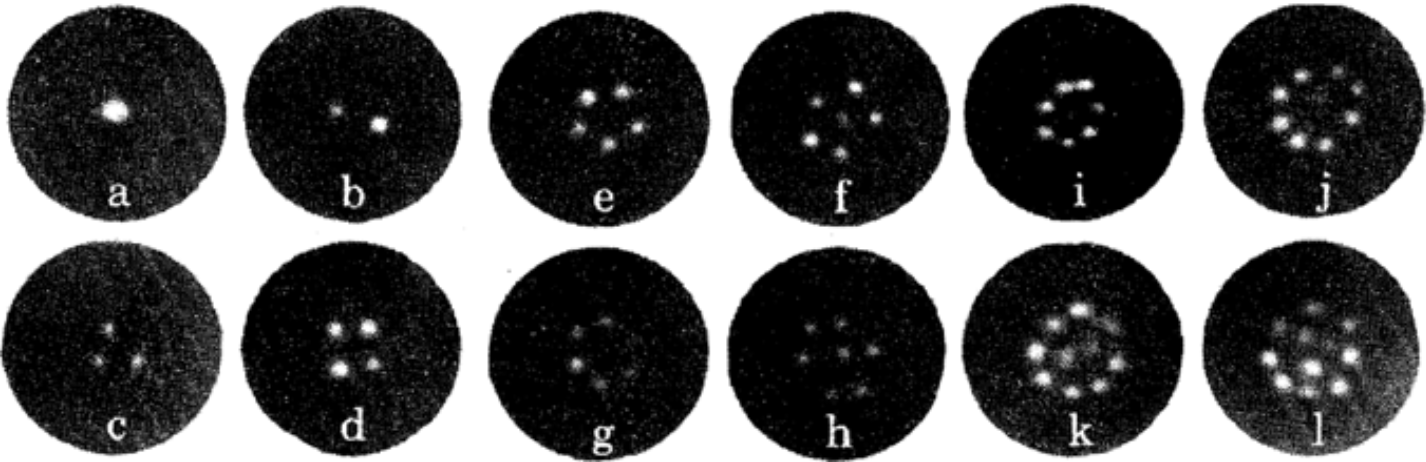
\includegraphics[width=\linewidth]{intro/packard}
\caption{\label{fig:hevorts} Results of the superfluid helium experiments of Packard \cite{PhysRevLett.43.214}, with (a-l) corresponding to increasing rotation velocities of the helium II container. Vortex line position is marked by the glowing dots.}
\end{figure}

\subsection{Solitons}
Solitons are a non-linear localised excitation, supported by the one dimensional GPE. Soliton solutions contain localised propagating wavepackets that are self-reinforcing due to the non-linearity of the system balancing dispersive effects. When in a homogeneous medium they travel at zero or finite constant speed, and have the property that they undergo non-destructive collisions. There are two species of soliton, bright \cite{PhysRevA.62.063611} and dark solitons \cite{PhysRevA.62.063610}. Their behaviour in optics, leading to a bright collection or dark absence of light, is the origin of these names. Solitons are an active area of research in several diverse areas of non-linear mathematics and physics \cite{drazin1989solitons,remoissenet2013waves}, and are well known for their applications in optical and fluid systems \cite{yu_kivshar_1998}. For these reasons solitons have been of great interest \cite{kevrekidis2007emergent,1751-8121-43-21-213001} since the first experimental realisation of atomic BECs.

In three-dimensional BECs, solitons take the form of solitonic waves, but are not solitons in the strict mathematical sense; the structures are unstable and proceed to decay \cite{Burger99,PhysRevA.62.053606,PhysRevA.65.043612,Tikhonenko96}. In weakly-interacting BECs with quasi-1D geometries, however, solitons are stable and have been observed with long lifetimes and with behaviour in agreement with numerical simulations \cite{PhysRevLett.101.120406}.

\subsubsection{Bright solitons}
Bright solitons arise in fluid \cite{Russell45}, plasma \cite{PhysRevLett.37.693,PhysRevLett.33.886}, acoustical \cite{naugolnykh1998nonlinear}, and optical physics \cite{agrawal2001nonlinear} and can be easily pictured by the classical example of a hump travelling along the surface of shallow water, as first reported in 1845 \cite{Russell45}. The non-dispersal and destruction-less collision properties of bright solitons make them particularly important in applications for optical communications \cite{hasegawa1995solitons}.

Bright solitons are supported in condensates for the case of effectively attractive interactions ($a_s < 0$) \cite{PhysRevA.62.063611}, were first generated and experimentally observed with lithium \cite{Strecker02,Khaykovich1290} in quasi-one-dimensional traps.

\subsubsection{Dark solitons}
In general, dark solitons are less prevalent than the bright species, but are of particular interest in the context of weakly-interacting BECs as they are are formed in the case of repulsive interactions ($a_s > 0$) \cite{PhysRevA.62.063610}. They consist of a density dip and phase slip \cite{dodd1982solitons} of varying size, depending on the speed of the soliton propagation. Dark solitons were first realised in 1987 in non-linear optics \cite{Emplit87}, followed by their creation in shallow liquids \cite{PhysRevLett.64.1518}, as discrete mechanical standing waves \cite{PhysRevLett.68.1730}, and in magnetic films \cite{PhysRevLett.70.1707}.

More recently, dark solitons have been engineered in repulsive atomic BECs in a controlled manner through phase imprinting methods \cite{Denschlag97,Burger99,PhysRevLett.86.2926,PhysRevLett.101.120406} and by perturbing the condensate density. They have also been produced through dynamical processes \cite{Weller08,PhysRevLett.99.160405}, such as by sweeping a laser beam through the condensate \cite{PhysRevLett.99.160405}. 

Dark solitons that have been generated in higher than quasi-1D geometries have been observed to decay into vortex rings \cite{PhysRevLett.86.2926,Dutton27072001,Shomroni09}, due to their known instability to transverse excitations.


\section{Quantum turbulence}
Classical turbulence is a complicated flow regime characterised by chaotic and highly irregular flow and the appearance of unsteady vortices on many length scales interacting with one another. In classical isotropic turbulence, most of the kinetic energy is contained in large-scale structures and is distributed following the famous Kolmogorov energy spectrum \cite{davidson2004turbulence}.

{\it Quantum} turbulence is a state dominated by an irregular tangle of quantised vortex lines. The quantised circulation and inviscid flow characteristics of superfluidity provides a simplified platform to study complicated vortex dynamics in general, and so the nature of turbulence in superfluids is the subject of much experimental and theoretical study \cite{Bradley11,skebek12,PhysRevLett.110.014502,barenghi_skrbek_14,PhysRevLett.115.155303}. Despite the fundamental differences between superfluids and classical fluids, the observations of Kolmogorov energy spectra in superfluid turbulence are suggestive of a deep connection between them \cite{barenghi_skrbek_14}. 

\subsection{Turbulence in helium II}
Quantum vortices are carriers of vorticity in superfluids and play an important role in the behaviour of the superfluid component of helium II. They have been experimentally and theoretically studied in helium II from around 1950 \cite{Donnelly}, but clearly visualising the three dimensional nature of individual vortex lines and reconnections remained a challenge until fairly recently \cite{Bewley09,Fonda12}: the large normal fluid component and a vortex core size of only a few Angstr\"oms limits visualisation techniques.

A large disordered collection of vortex lines is thought to be the driving force of the turbulence. However, within the tangle the vortex core size is small compared to the average inter-vortex spacing. For this reason the standard method of modelling of vortex dynamics at large-scales is handled by approximating the vortices as infinitesimally thin vortex filaments, with motion described by the Biot-Savart law \cite{barenghi_donnelly_01}. The limitation of the vortex filament model is that all phenomena that occur on the length-scale of the vortex core (of which we are interested in) is lost. Features like vortex reconnection can be manually introduced into this model \cite{barenghi_donnelly_01}, but the full microscopic description is lost.

On the other hand, the GPE model for a weakly-interacting Bose gas provides a microscopic model of helium II on a qualitative level. As already discussed, the strongly-interacting helium atoms, existence of high momenta rotons, and relatively low fraction of condensed helium atoms limits the accuracy of the model. Nevertheless, the GPE excels at describing the micro-scale phenomena such as vortex nucleation \cite{frisch92}, reconnections \cite{PhysRevLett.71.1375, PhysRevLett.76.4745}, sound emission \cite{leadbeater,PhysRevA.69.053601}, and Kelvin wave excitation, and so we will use the GPE at various points throughout this thesis to model helium II dynamics.

Typically turbulence in helium II is generated using mechanical methods, creating turbulence with oscillating obstacles, including grids \cite{Davis2000}, wires \cite{Guenault1986,Bradley2011,Fisher2001}, spheres \cite{Schoepe1995} and others \cite{Blaauwgeers2007,Bradley2012,Tabeling1998,Salort,VinenSkrbek2008}. Methods without the use of oscillating structures have been also been devised, such as the use of heat flux \cite{Vinen114} or container spin-down \cite{PhysRevLett.99.265302}, to generate turbulence . A mutual friction \cite{Donnelly} couples the normal fluid and superfluid components, and at finite temperature leads to a dissipation of the resulting turbulent vortex tangle. In the limit of very low temperatures the mutual friction tends to zero. It is expected that in this limit Kelvin wave excitations \cite{leadbeater,PhysRevA.69.053601} and vortex reconnections leads to dissipation via sound waves, but the entire mechanism is not yet fully understood \cite{PhysRevB.61.1410}.

\subsection{Turbulence in BECs}

Weakly interacting atomic BECs present a key improvement over helium II superfluidity for the study of quantum turbulence. Although the spatial extent of BECs support much fewer vortices than for superfluid helium, the structure of individual vortices and their turbulent dynamics can be experimentally resolved much easier. This is due to the relatively large vortex core size, on the scale of a micron, available to atomic BECs and the fact that the state of the entire atomic gas can be readily visualised through imaging techniques. Expansion imaging has provided a technical leap in this area, allowing individual vortex cores and reconnection events to be directly observed \cite{PhysRevLett.84.806,Raman01,kwon_moon_14}. Improved real time and non-destructive imaging of condensates is now possible \cite{Freilich2010} by out-coupling of a small representative fraction of the gas for each image, allowing for observation of quantum vortex trajectories. A further recent improvement in this area \cite{powis} has allowed for the imaging of vortex polarity as well as its location in space. These technical leaps in imaging have made atomic condensates an extremely attractive medium for exploring quantum vortex turbulence. 

The range of length scales available to classical turbulence and superfluid helium turbulence far outshines those currently available to atomic BECs, and much theory of classical turbulence is defined by the distribution of kinetic energy over the large number of length scales available. Nevertheless, numerical studies show quantum turbulence can distribute the kinetic energy in an atomic condensate in agreement with Kolmogorov's $k^{-5/3}$ law \cite{Nore,Kobayashi,PhysRevLett.103.084501}.

\section{Thesis overview}
An outline of the thesis structure and a brief description of each chapter is given in this section. The thesis is split into three main parts. Part I introduces the formalism, models and numerical tools that we go on to use in part II to model quantum fluids and generate numerical results. Part III is a collection of appendices. The following publications feature partially some of the results shown in the thesis, and the collaborative contributions are highlighted here.
\begin{itemize}
	\item Quantum analogues of classical wakes in Bose-Einstein condensates\\
	{\footnotesize G. W. Stagg, N. G. Parker and C. F. Barenghi, J Phys B: At. Mol. Opt. Phys. {\bf 47} 095304 (2014)}
	\item Generation and decay of two-dimensional quantum turbulence in a trapped Bose-Einstein condensate\\
	{\footnotesize G. W. Stagg, A. J. Allen, N. G. Parker and C. F. Barenghi, Phys. Rev. A {\bf 91}, 013612 (2015)}
	\item Classical-like wakes past elliptical obstacles in atomic Bose-Einstein condensates\\
	{\footnotesize G. W. Stagg, A. J. Allen, C. F. Barenghi, N. G. Parker, J. Phys.: Conf. Ser. {\bf 594} 012044 (2015)}
	\item Critical velocity of a finite-temperature Bose gas\\
	{\footnotesize G. W. Stagg, R. W. Pattinson, C. F. Barenghi, N. G. Parker, Phys. Rev. A {\bf 93}, 023640 (2016)}
	\item A superfluid boundary layer\\
	{\footnotesize G. W. Stagg, N. G. Parker, C. F. Barenghi, arXiv:1603.01165 (2016)}
\end{itemize}

\subsubsection{Part I - Introduction and Theory}
Chapter 1 introduces the concept of Bose-Einstein condensation, superfluidity, and the nature of quantum turbulence in weakly interacting atomic condensates and superfluid liquid helium.

Chapter 2 describes the theoretical concepts and mean-field methodology that allows us to efficiently model a dilute, weakly interacting atomic Bose gas at zero and finite temperatures. We describe the Gross-Pitaevskii equation (GPE), a non-linear Schr\"odinger equation used to model condensates at zero temperature, and go on to extend the GPE to take into account finite temperature effects through phenomenological damping or the classical-field method. We detail some of the consequences of the model, such as quantised circulation, and show various initial conditions and simple solutions of the GPE.

Chapter 3 details the theory and implementation of various numerical procedures we use to generate the simulations and results shown in part II. The time-stepping numerical solver is described, followed by an extensive description of the vortex locating and tracking subroutines. Finally a method is described for the filtering of the thermal part of the field when using the classical-field method.

\subsubsection{Part II - Numerical Studies}
Part II consists of a selection of the numerical simulations we have performed, interpretations of the results and any applications to real experimental systems. Chapter 4 extends recent studies of moving obstacles in superfluids, a system mimicking a well known problem for classical viscous flows. We present numerical simulations of classical-like wakes, consisting of vortex clusters, generated by the presence of elliptical obstacles.

Chapter 5 was motivated by the recent experimental work of Kwon {\it et al.} \cite{kwon_moon_14}. We model their experimental set up in which a trapped condensate is translated past an obstacle, and study the decay of the resulting 2D quantum turbulence and vortex annihilation events. Communications with Y. Shin and A. Cidrim were helpful in the interpretation of the numerical simulations shown in this chapter.

Chapter 6 was motivated by further work of Kwon {\it et al.} \cite{kwon_2015a}, highlighting the need to extend the study of the critical velocity for vortex nucleation to finite temperatures. We use classical field methods to simulate finite temperature homogeneous Bose gases. We simulate the gas from a strongly non-equilibrium initial distribution, and classify the nature of the resulting turbulent vortex tangle. The previous numerical work of A. J. Youd was helpful in the development of our classical-field code used in this chapter.

Chapter 7 is inspired by recent experimental studies in helium II, generating turbulence with oscillating obstacles such as wires, spheres and grids \cite{Davis2000,Guenault1986,Bradley2011,Fisher2001,Schoepe1995,Blaauwgeers2007,Bradley2012,Tabeling1998,Salort,VinenSkrbek2008}. We simulate a quantum fluid in the presence of a real rough boundary obtained via atomic force microscopy \cite{Lawson}, with data kindly provided by C. R. Lawson. We find surprising evidence suggesting the formation of a thin `superfluid boundary layer' consisting of vortex loops and rings.

In Chapter 8 we briefly review the main conclusions of the work shown in the thesis and discuss opportunities for further research in the area.

\subsubsection{Part III - Appendix}
Part III is a collection of appendices. Appendix A consists of various detailed derivations relevant to the theoretical modelling of an atomic BEC. Appendix B contains definitions of relevant quantities in our quantum fluid simulations. Appendix C is a collection of numerical algorithms that we have used.



\end{chapter}
